% ---------------------------------------- %
%              BRADY RIPPON                %
% ---------------------------------------- %
%            LATEX CHEET SHEET             %
% ---------------------------------------- % 

%% NOTE: If you click anywhere on the PDF, %%
%% the code to the left will jump to that  %%
%% spot to make navigating easier.         %%

\documentclass[12pt]{article}
% Controls the font and type of document --
% "article" is best for scientific journals 
% and shorter reports

% ---------------------------------------- %
%            PACKAGES & TOOLS              %
% ---------------------------------------- % 

% There are a ton of packages in LaTeX that help
% you do cool things. These are a few of the ones 
% I use.

\usepackage[margin=1in]{geometry} 
\usepackage{amsmath,amsthm,amssymb}
\usepackage{tasks}
\usepackage{enumerate}
\usepackage{float}
\usepackage{physics}
\usepackage{multirow,multicol}
\usepackage{hhline}
\usepackage{enumitem}
\usepackage{graphicx}
\usepackage{tikz}
\usepackage{pstricks-add}
\usepackage{mathtools}
\usepackage{booktabs}
\usepackage{breqn}

\newcommand{\N}{\mathbb{N}}
\newcommand{\Z}{\mathbb{Z}}

% This next section of code isn't really necessary, 
% but I use it a lot to format questions 
% neatly in homework assignments.
 
\newenvironment{theorem}[2][Theorem]{\begin{trivlist}
\item[\hskip \labelsep {\bfseries #1}\hskip \labelsep {\bfseries #2.}]}{\end{trivlist}}
\newenvironment{lemma}[2][Lemma]{\begin{trivlist}
\item[\hskip \labelsep {\bfseries #1}\hskip \labelsep {\bfseries #2.}]}{\end{trivlist}}
\newenvironment{exercise}[2][Exercise]{\begin{trivlist}
\item[\hskip \labelsep {\bfseries #1}\hskip \labelsep {\bfseries #2.}]}{\end{trivlist}}
\newenvironment{reflection}[2][Reflection]{\begin{trivlist}
\item[\hskip \labelsep {\bfseries #1}\hskip \labelsep {\bfseries #2.}]}{\end{trivlist}}
\newenvironment{proposition}[2][Proposition]{\begin{trivlist}
\item[\hskip \labelsep {\bfseries #1}\hskip \labelsep {\bfseries #2.}]}{\end{trivlist}}
\newenvironment{corollary}[2][Corollary]{\begin{trivlist}
\item[\hskip \labelsep {\bfseries #1}\hskip \labelsep {\bfseries #2.}]}{\end{trivlist}}
\newenvironment{problem}[2][Problem]
{\begin{trivlist}
\item[\hskip \labelsep {\bfseries #1}\hskip \labelsep {\bfseries #2.}]}{\end{trivlist}}
\newenvironment{question}[2][Question]
{\begin{trivlist}
\item[\hskip \labelsep {\bfseries #1}\hskip \labelsep {\bfseries #2.}]}{\end{trivlist}}
\newenvironment{solution}[2][\underline{Solution}]
{\begin{trivlist}
\item[\hskip \labelsep {\bfseries #1}\hskip \labelsep {\bfseries #2}]}{\end{trivlist}}
% Allows you to make custom lists. You can take the 
% period out of "\bfseries #2." to eliminate
% the period from the output (see: Lists)


\newenvironment{tightcenter}{%
  \setlength\topsep{0pt}
  \setlength\parskip{0pt}
  \begin{center}
}{%
  \end{center}
}
 
\begin{document}
 
% ---------------------------------------- %
%            START OF DOCUMENT             %
% ---------------------------------------- %

\title{\LaTeX \text{} Cheat Sheet}
\author{Your Name} 
% You can use the following to add a header under your name:
% ** \author{Your Name \\ Second Header} **

\maketitle
% Making a title in this way will also include 
% the current date.


% ---------------------------------------- %
%            TEXT ORGANIZATION             %
% ---------------------------------------- %

\section*{Text Editing}

Just typing normal text will place what you type directly into the document. The text starts indented automatically. 

Manually typing in a space in your code will create a new indented paragraph. 
\newline
Using the "newline" command will create a new paragraph that is not indented.

\begin{tightcenter}
\line(1,0){465}
\end{tightcenter}
% I use this to create nice horizontal lines 
% across the entire page.

\section{Section 1}
\subsection{Subsection 1}
\subsubsection{Subsubsection 1}
\section{Section 2}
% Creates a list of numbered sections

\section*{Section 1}
\subsection*{Subsection 1}
\subsubsection*{Subsubsection 1}
\section*{Section 2}
% Creates a list of unnumbered sections

\begin{tightcenter}
\line(1,0){465}
\end{tightcenter}

The design of the text can be changed on the fly. You can create \textbf{bold text}, \textit{italic text}, \textsc{small caps text}, \textsl{slanted text}, \texttt{typewriter text}, and \textrm{times new roman text}. The text size can also be change as \tiny{tiny}, \small{small}, normal, and increasingly larger sizes: \large{large}, \Large{large}, \LARGE{large}, \huge{large}, \Huge{large} \normalsize{.}
% If you don't use "\normalsize" here the rest
% of the document text will be the last size
% you used.

\begin{tightcenter}
\line(1,0){465}
\end{tightcenter}
\newpage
% Skips to the top of the next page


% ---------------------------------------- %
%              MAKING LISTS                %
% ---------------------------------------- %

\section*{Lists}

\begin{enumerate}
% The "\item" commands signals LaTeX to create the
% next item of the list inside "\enumerate"
\item The first item in the default numbered list

% You can nest lists within lists.
% When you do this, you usually want to specify 
% the label of your list. LaTeX will just pick 
% something automatically if you don't.
\begin{enumerate}[label=(\alph*)]
% Makes a list of lowercase letters in parentheses
\item First lettered item
\begin{enumerate}[label=\roman*.]
% Nests another list, this time with roman 
% numerals followed by a period.
\item First roman numeral item
\item Second roman numeral item
\end{enumerate}
\item Second lettered item
\end{enumerate}

\item The second item in the default numbered list
\item The third item in the default numbered list
\end{enumerate}

\begin{tightcenter}
\line(1,0){465}
\end{tightcenter}

% You can also make symbol lists with the "\itemize"
% command. These lists default as bullets. 

% Also, you can nest a "\multicol" command within
% any list to make the list format in a designated 
% number of columns. Notice the order of the 
% items (LaTeX fills an entire column before 
% moving on to the next one). 
\begin{itemize}
\begin{multicols}{2}
\item[$\square$] First thought
\item Second thought
\item Third thought
\item[$\blacksquare$] Fourth thought
\end{multicols}
\end{itemize}

\begin{tightcenter}
\line(1,0){465}
\end{tightcenter}

% This commands refer to the "\trivlist" commands 
% from the top of the document, which each 
% essentially created a new command to use. 
\begin{question}{1}
Your question.
\end{question}

% Make the same list but skip a line
\begin{problem}{4} \text{} \newline
Your problem
\end{problem}

% Changing the format of the list.
% See "\trivlist" for "solution" at top to
% observe what was edited to make these changes.
\begin{solution}{(15)}
Your solution
\end{solution}


\begin{tightcenter}
\line(1,0){465}
\end{tightcenter}

\newpage

% ---------------------------------------- %
%            MATH AND EQUATIONS            %
% ---------------------------------------- %

\section*{Math Mode and Equations}

% LaTeX default types in "text mode," so a lot 
% of math symbols will create errors if you
% try to type them normally. You can manually 
% switch to "math mode" by inserting a $. 
% You can leave math mode by inserting another $. 
% This can be done in the middle of a line of 
% text if you want.

Some useful \LaTeX\text{} math operations include: 
% Find the number in the comments of the code to see
% how each expression is written
\begin{enumerate}
\begin{multicols}{3}
% 1. %
\item $X^{10}$
% 2. %
\item $X_{10}$
% 3. %
\item $X_{10}^{10}$
% 4. %
\item $f'(x)$ 776767676 something here
% 5. %
\item $X \rightarrow Y \Rightarrow Z$
% 6. %
\item $Pr(A \cup B \mid C \cap D)$
% 7. % -- if you have a big fraction to put in 
%      -- parentheses, it will look better if you
%      -- put them inside bigger parentheses.
%      -- Also works for brackets and braces.
\item $\Bigg(\bigg(\Big(()\Big)\bigg)\Bigg)$
% 8. %
\item $\frac{x + 7}{2x - 5}$
% 9. % -- "cfrac" won't condense the fraction to
%      -- the size of the line you're using
\item $\cfrac{x + 7}{2x - 5}$
% 10. %
\item $\sqrt{x}$ and $\sqrt[3]{x}$
% 11. %
\item $\sum_{i=0}^{n}$
% 12. %
\item $\int_{x=0}^{1}f(x)\partial x$
% 13. % 
\item $< , > , \geq , \leq , \neq, \pm, \therefore $
% 14. %
\item $\binom{n}{k}$
% 15. % -- preference which one you use
\item $\overline{X}$ and $\bar{X}$
% 16. %
\item $\infty$
% 17. %
\item $\left|X - 2\right|$
% 18. %
\item $\boxed{y = mx + b}$
% 19. %
\item $\hat{X}$
% 20. %
\item $X \sim N(\mu, \sigma^{2})$
% 21. %
\item $\pi \approx 3.14$
% 22. % 
\item $\sin(x)$ and $\cos(x)$
% 23. %
\item $X \cdot Y$
% 24. % -- As an aside, using "\left(\right)"
%       -- and putting an equation inside the
%       -- parentheses will make LaTeX re-size
%       -- the parentheses automatically.        
\item $\left.\bigg(\cfrac{x}{2} \bigg)\right\vert_{0}^{1}$
% 25. % -- bold math font
\item $\mathbf{X}$
% 26. % -- make a symbol bold font
\item $\boldsymbol{\pi}$
% 27. -- math calligraphy font
\item $\mathcal{X}$ 
% 28. % -- blackboard bold font
\item $\mathbb{X}$
\end{multicols}
\end{enumerate}

\textbf{For all Greek symbols:} http://web.ift.uib.no/Teori/KURS/WRK/TeX/symALL.html

\newpage

% Using math mode in line with your text all 
% the time will make your work very cluttered. 
% It's usually best to divide your math work 
% up separately in one of the following formats.

\begin{tightcenter}
\line(1,0){465}
\end{tightcenter}

% This will make an equation with a label 
% in the right margin.
% The (1) is not the same as the "\label"
% command. The label in the margin is a count
% of how many equations you've used in the 
% document so far. The "\label" command is 
% used in your code to reference the equation.
\begin{equation} \label{eq3}
\lim\displaylimits_{x \rightarrow \infty}f(x) = 0
\end{equation}

% Using "$$" instead of "$" will also enter
% math mode but will scale all the math to
% the appropriate font and center the work 
% on its own line.
$$ \cfrac{X-n\mu_{x}}{\sigma_{x}\sqrt{n}} = \cfrac{X-12(16)}{1\sqrt{12}} $$

% Notice that if you are currently in math
% mode (the "\align" starts math mode), you
% can't type text anymore. To add words in
% an equation, use the "\text" command.
$$ Z = \cfrac{\overline{x} - \mu_{0}}{\sigma / \sqrt{n}} \rightarrow \text{ If }\left| Z \right| > z_{1-\alpha/2}\text{, reject }H_{0} $$

% Another example
$$ Pr\Big(\lim\displaylimits_{n \rightarrow \infty} \overline{X}_{n} = \mu \Big) = 1 \text{, so } \overline{X}_{n} \xrightarrow{a.s.} \mu $$

% To make aligned equations, most places
% will say to use the "\equarray" command, 
% but you're better off using the "\align"
% command instead. It solves a couple 
% formatting issues you might run into
% with "\equarray" and doesn't break
% equations across pages, which "\equarray"
% does. 
\begin{align*}
    \text{var}(U_{1})&= \text{var}(aY_{1} + bY_{2})\\
    &= \text{var}(aY_{1}) + \text{var}(bY_{2}) + 2\text{cov}(aY_{1},bY_{2})\\
    &= \text{var}(aY_{1}) + \text{var}(bY_{2}) + 0&& (Y_{1} \text{ \textit{and} } Y_{2} \text{ \textit{uncorrelated})} \\
    &=a^{2} \cdot \text{var}(Y_{1}) + b^{2} \cdot \text{var}(Y_{2}) && (a = b = 1)\\
    &=\text{var}(Y_{1}) + \text{var}(Y_{2}) \\
    &= \sigma_{1}^{2} + \sigma_{2}^{2}\\
\end{align*}
% The "&" signs designate where your 
% alignments go. Anything after the first 
% "&=" will appear in the same spot down
% the equation. You can add "&&" at the 
% end of any of those lines to add aligned
% in-line comments as you go.

\begin{tightcenter}
\line(1,0){465}
\end{tightcenter}

% piece-wise functions
\[
f_{XY}\textbf{(}x,y\textbf{)}=
% The "\cases" command allows you to list
% all the possible pieces to the function,
% with the individual domains separated 
% and aligned by the "&." 
\begin{cases}
xy/96, &0 < x < 4\text{ , }1<y<5\\
0, &\text{elsewhere}
\end{cases}
\]

\begin{tightcenter}
\line(1,0){465}
\end{tightcenter}

% Matrices
$$
A^{T} = \left[
\begin{matrix}
a_{11} & 0 & \ldots & a_{1n}\\
0 & a_{22} & \ldots & a_{2n}\\
\vdots & \vdots & \ddots & \vdots\\
0 & 0 &\ldots & a_{nn}
\end{matrix}
\right]
$$

$$
M_{n \times 1} = \left(
\begin{matrix}
\mu_{1}\\
\mu_{2}\\
\vdots\\
\mu_{n}
\end{matrix}
\right)
$$

\begin{tightcenter}
\line(1,0){465}
\end{tightcenter}

\newpage

% ---------------------------------------- %
%             MAKING A TABLE               %
% ---------------------------------------- %

\section*{Tables and Figures}

\begin{table}[H]
% This [H] fixes the float point of the table
% to immediately after the text before it
% Leaving this out might cause the table to float 
% to a weird spot on the page. The [H] stands
% for 'here.' You could also use [b] (bottom)
% or [t] (top). 
\large 
% Picks the size of the table
\centering 
% Orients the table
\begin{tabular}{|c|c|c|}
% Determines how many columns you have.
% "c" has no lines separating it from other columns
% "|c|" has lines on both sides
\hline
% Creates a horizontal line below this row
\multirow{2}{*}{Evaluation} & \multicolumn{2}{c|}{Disease Status} \\
% Uses the "multirow" and "multicolumn" packages 
% to combine cells 
\hhline{~--}
% Uses "hhline" package to create a custom "hline"
% Otherwise the hline will cut through all cells 
 & HIV$^{+}$ & HIV$^{-}$ \\
\hline
Minority & n$_{1,1}$ & n$_{1,2}$  \\
\hline 
Non-minority & n$_{2,1}$ & n$_{2,2}$ \\
\hline
\end{tabular}
\end{table}

% The "multicols" function can be used to fit two
% tables side-by-side.
\begin{multicols}{2}
\begin{table}[H]
\large
\centering 
\begin{tabular}{|c|c c|c|c|}
\hline
$\left| d_{i} \right|$ & $f_{i}^{+}$ & $f_{i}^{-}$ & Range & Rank \\
\hline \hline
% Two "hlines" will make two consecutive lines
% and create an aesthetic space if placed 
% in the middle of the table.
0.3 & 1 & 0 & - & 1 \\
\hline
1.8 & 0 & 1 & - & 2 \\
\hline 
2.2 & 1 & 0 & - & 3\\
\hline
2.7 & 0 & 1 & - & 4 \\
\hline
3.5 & 1 & 0 & - & 5\\
\hline
4.5 & 0 & 1 & - & 6 \\
\hline
4.8 & 1 & 0 & - & 7 \\
\hline 
5.4 & 1 & 1 & 8--9 & 8.5\\
\hline
5.8 & 1 & 0 & - & 10\\
\hline
5.9 & 0 & 1 & - & 11\\
\hline
6.0 & 1 & 0 & - & 12 \\
\hline
\end{tabular}
\end{table}
\begin{table}[H]
\large
\centering 
\begin{tabular}{|c|c c|c|c|}
\hline
$\left| d_{i} \right|$ & $f_{i}^{+}$ & $f_{i}^{-}$ & Range & Rank \\
\hline \hline
6.7 & 1 & 0 & - & 13 \\
\hline 
9.6 & 1 & 0 & - & 14\\
\hline
10.3 & 0 & 1 & - & 15\\
\hline
11.5 & 1 & 0 & - & 16 \\
\hline
12.2 & 1 & 0 & - & 17\\
\hline
12.6 & 0 & 1 & - & 18 \\
\hline
13.9 & 1 & 0 & - & 19 \\
\hline 
14.2 & 1 & 0 & - & 20\\
\hline
18.0 & 1 & 0 & - & 21\\
\hline
18.6 & 1 & 0 & - & 22\\
\hline
21.7 & 1 & 0 & - & 23 \\
\hline
\end{tabular}
\end{table}
\end{multicols}

% An image or figure can be added in the same
% way by using the "figure" command. First, add
% the file to your LaTeX document. In the top-left
% corner, PROJECT -> Files... -> Upload from
% Computer -> select the file.
\begin{figure}[H]
\centering
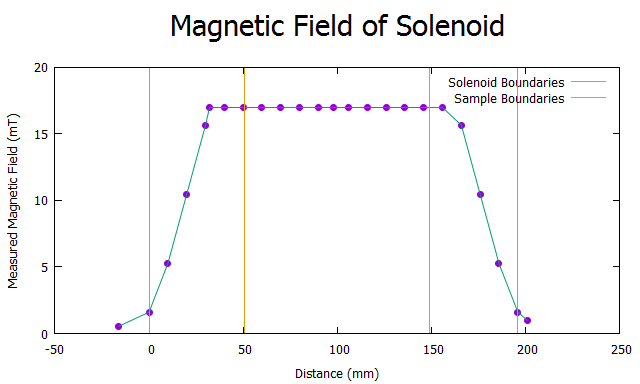
\includegraphics[width=.75\textwidth]{Solenoid_Hall_Probe3.png}
% You can change the size of the image as 
% it will appear in the document.
% Type the name of the figure exactly as it 
% appears in the file directory to the left.
\caption{Measured magnetic field by position relative to solenoid left edge (x = 0) and SF-57 glass rod (sample).}
\label{figure:1}
% Adding a caption and label is optional to the
% "figure" command. Just get rid of these two
% commands if you don't want them.
\end{figure}
% You can place two figures next to each other
% just like the tables with "multicols."

\newpage

% ---------------------------------------- %
%             DISPLAYING CODE              %
% ---------------------------------------- %

\section*{Displaying Code in \LaTeX}

% Exact code cannot be copy and pasted into 
% LaTeX, as the formatting of the two programs
% will almost definitely conflict. 

% Instead, you can use the "verbatim" command to 
% copy and paste while maintaining the format
% of a source outside of LaTeX. Anything 
% inside this command will be in red font.
\begin{verbatim}
# Filename: ProgrammingBasics.R
 
# ---Simple Calculations---
2 + 3
 
x <- 2
y <- 3
x + y
x * y
 
# ---Data Structures---
 
# Vectors
workshop <- c(1, 2, 1, 2, 1, 2, 1, 2)
print(workshop)
workshop
 
gender <- c("f", "f", "f", NA, "m", "m", "m", "m")
q1 <- c(1, 2, 2, 3, 4, 5, 5, 4)
q2 <- c(1, 1, 2, 1, 5, 4, 3, 5)
q3 <- c(5, 4, 4,NA, 2, 5, 4, 5)
q4 <- c(1, 1, 3, 3, 4, 5, 4, 5)
 
# Selecting Elements of Vectors
q1[5]
q1[ c(5, 6, 7, 8) ]
q1[5:8]
q1[gender == "m"]
mean( q1[ gender == "m" ], na.rm = TRUE)
\end{verbatim}


%%%%%%%%%%%%%%%%%%%%%%%%%%%%%%%%%%%%%%%%%
%%%%%%%%%%%%%%%%%%%%%%%%%%%%%%%%%%%%%%%%%

\end{document}